\section{Stateless Tracking}
\label{sec:stateless-tracking}

Under stateless tracking (see \autoref{tab:appendix-stateless-tracking}), trackers do not rely on a stored state (\ie{}, ID) in the browser to track a user, and instead collect artifacts of the user's behavior, browser, or hardware to generate a fingerprint to correlate a user across sites and sessions.
% 
Analysis of real-world fingerprints and entropy computations have revealed that some attributes can contribute a lot more to the uniqueness of users than others, leading to the identification of a specific user with high certainty~\cite{eckersleyHowUniqueYour2010,laperdrixBeautyBeastDiverting2016,gomez-boixHidingCrowdAnalysis2018,bacis2024assessing}. 
%
% \autoref{tab:appendix-stateless-tracking} summarizes different mechanisms and defenses.


%%
\subsection{Fingerprinting and Types}

Fingerprinting corresponds to the gathering of information on users’ behavior, browsers, and devices in real-time with the goal of identifying users. 
%
\autoref{fig:stateless-tracking} depicts how fingerprinting works; through HTTP headers and calls to specific JavaScript APIs, a website can collect a wide range of information on the user's behavior (\eg{} mouse movements, keystrokes, and clicking), browser (\eg{} browser version, screen size, installed fonts, GPU model, timezone and preferred languages), and configuration of the underlying OS and the hardware. 
% 
Its use for tracking purposes has been hard to detect and block, as fingerprinting can be used (1) constructively, to identify user-impersonating actors such as bots or fraudsters, and (2) destructively to identify and track users who wish to remain anonymous (see~\autoref{sec:need-for-fingerprinting}). 
%
Additionally, it is difficult to prevent as users exhibit the same behavior and retain the same device over time, which can result in certain stable fingerprinting attributes.
%
Several types of fingerprinting techniques exist based on the nature of the collected attributes.
% Among them, browser fingerprinting has been the most studied and widely used mechanism in context of the web. 

\begin{figure}[htbp]
    \centering
    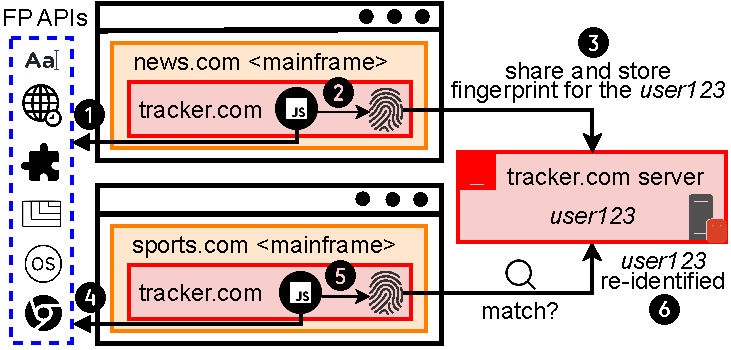
\includegraphics[width=0.85\linewidth]{figures/tracking-mechanisms-fingerprinting.pdf}
    \caption{Stateless Tracking via Fingerprinting.}
    \label{fig:stateless-tracking}
\end{figure}

%%
\para{Browser Fingerprinting.} 
%
Relying on browser-based APIs to collect information about configurations of the browser, device or the underlying OS to generate a fingerprint is referred to as browser fingerprinting.
%
Since the first academic work on browser fingerprinting in 2009~\cite{mayerAnyPersonPamphleteer2009}, researchers have studied: its impact on privacy~\cite{eckersleyHowUniqueYour2010}, its use with other tracking techniques~\cite{fouadMyCookiePhoenix2022} and in real world applications~\cite{aminazadWebRunner20492020, wuHimManyFaces2023}, its detection~\cite{iqbalFingerprintingFingerprintersLearning2021, boussahaFPtracerFinegrainedBrowser2024}, abusable browser APIs~\cite{bahramiFPRadarLongitudinalMeasurement2022, suAutomaticDiscoveryEmerging2023, senolDoubleEdgedSword2024}, and user protections~\cite{vastelFpScannerPrivacyImplications2018}. 
%
The Electronic Frontier Foundation’s Panopticlick project \cite{effpanopticlick} provided one of the earliest large-scale empirical demonstrations of browser fingerprintability and associated risks. 
% and has been influential in characterizing real-world browser fingerprinting risks.
%
In 2013, fingerprinting was observed on $\sim$1\% of the top 10K websites~\cite{nikiforakisCookielessMonsterExploring2013} and $\sim$400 of the top 1M websites~\cite{acarFPDetectiveDustingWeb2013}. 
%
Over the years, a variety of techniques have been used to measure browser fingerprinting~\cite{acarWebNeverForgets2014,englehardtOnlineTracking1millionsite2016,olejnikBatteryStatusNot2017,dasWebsSixthSense2018}, with two general trends being: its higher adoption by third-parties and its expansion to a diverse set of browser APIs over the years. 
%
By 2021, fingerprinting scripts were found to be present on 10\% of the top 100K websites, with more popular ones having a higher incidence (\ie{}, 30\% of the top 1,000)~\cite{iqbalFingerprintingFingerprintersLearning2021}.
%
Importantly, browser fingerprints are not always stable enough to track users over time: 80\% of browser instances change fingerprints in less than 10 days~\cite{vastelFPSTALKERTrackingBrowser2018}. 
%
Trackers not only link fingerprints as they evolve, but also combine and persist them with \textit{stateful} techniques, rendering the technique effective even in browsers that partition third-party access to stateful APIs (\autoref{sec:stateful-defenses}). 
%
A 2022 study measured a lower bound on this approach by detecting cookie respawning due to browser fingerprinting on 1,150 of the top 30K sites~\cite{fouadMyCookiePhoenix2022}.
%
Prior works have explored various browser-supported JavaScript APIs for fingerprinting such as Canvas~\cite{moweryPixelPerfectFingerprinting2012}, WebGL~\cite{caoCrossBrowserFingerprintingOS2017}, Audio API~\cite{englehardtOnlineTracking1millionsite2016}, the Battery Status API~\cite{olejnikLeakingBatteryPrivacy2016}, as well as font and device-class characteristics exposed through rendering and system metrics~\cite{fifield2015fingerprinting,bursztein2016picasso}.
%
Other recent works indicate that fingerprinting risks differ across demographics~\cite{berkeHowUniqueWhose2025} and that certain information contained in fingerprints could be limited without breaking the user experience~\cite{intumwayaseUARadarExploringImpact2023}.\\



%%
\para{Side-channel Fingerprinting.} 
% 
% Trackers may also exploit available browser APIs and resources to find new side-channels to fingerprint the user's browser or device. 
% %
% Besides browser fingerprinting techniques, researchers have demonstrated numerous side-channel approaches to track users.
%
Side-channel fingerprinting research has evolved from early demonstrations of unintended browser state leakage—such as history sniffing~\cite{weinbergStillKnowWhat2011}, cache abuse~\cite{shusterman2021prime+}, and favicon-based persistence~\cite{solomosTalesFaviconsCaches2021}—to increasingly systematic and automated analyses of cross-site information flows in modern browsers~\cite{knittelXSinatorcomFormalModel2021}. 
%
As defenses have closed individual leaks, subsequent work has shifted towards identifying newer classes of tracking vectors, leveraging timing~\cite{jinTimingBasedBrowsingPrivacy2022}, resource contention~\cite{snyderPoolPartyExploitingBrowser2023}, and feature exposure~\cite{aliNavigatingMurkyWaters2023} as more subtle fingerprintable signals within the browser. 
%
More recently, side-channel techniques have expanded beyond the browser’s internal state to external observables such as network metadata~\cite{leeNettrackGenericWeb2023} and physical signals~\cite{jeonImListeningYour2018}, enabling coarse tracking even under strong isolation or encryption assumptions. 
%
Together, this line of work has suggested a trajectory away from brittle single-mechanism attacks and toward compositional and cross-layer side channels that exploit performance optimizations, shared infrastructure, and user interactions. 
%
Generally, side-channel attacks are challenging to detect and could be equally difficult to mitigate.

%%
\para{Extension Fingerprinting.} 
%
This other side-channel approach aims at inferring the presence of specific extensions in user's browser~\cite{karamiCarnusExploringPrivacy2020}. 
%
Early studies~\cite{sjostenDiscoveringBrowserExtensions2017, gulyasExtendNotExtend2018, karamiCarnusExploringPrivacy2020} demonstrated how extensions contain specific resources (\eg{},~images, scripts) that can be referenced by web pages, thereby revealing their presence. 
%
Researchers have also explored behavioral extension fingerprinting~\cite{starovXHOUNDQuantifyingFingerprintability2017, karamiCarnusExploringPrivacy2020, solomosDangersHumanTouch2022, solomosEscapingConfinesTime2022, laperdrixFingerprintingStyleDetecting2021, agarwalPeekingWindowFingerprinting2024}, where an extension can be implicitly inferred through executional side-effects, and corresponding mitigations~\cite{karamiUnleashSimulacrumShifting2022, sanchez-rolaExtensionBreakdownSecurity2017} such as randomizing WARs, IDs, or classes~\cite{trickelEveryoneDifferentClientside2019}, and access control based extension loading~\cite{sjostenLatexGlovesProtecting2019}. 


%%
\para{Behavioral Fingerprinting.} 
%
% Behavioral fingerprinting involves using browser APIs and setting-up event listeners to record user's behavior (\eg{} mouse movements, keystrokes, click behavior, and other interaction patterns) on a website, that are known to be unique for a given user~\cite{leivaMyMouseMy2021}.
%
Early work on behavioral fingerprinting has shown that fine-grained interaction signals such as mouse movements can reliably distinguish users and support continuous or implicit authentication~\cite{zhengEfficientUserVerification2011,jorgensenMouseDynamicsBehavioral2011}, even in realistic adversarial settings~\cite{fereidooniAuthentiSenseScalableBehavioral2023}. 
%
Similarly, keystroke patterns from user's typing behavior can be used to reliably link a user across their devices~\cite{yuanCrossdeviceTrackingIdentification2018}.
%
Such behavioral signals are commonly used in bot detection and inference of user attributes from interaction traces~\cite{leivaMyMouseMy2021}. 


%%
\para{Hardware Fingerprinting.} 
%
Sanchez-Rola et al. demonstrated how JavaScript APIs can be used to construct a hardware fingerprint by analyzing the execution timing of instruction sequences~\cite{sanchez-rolaClockClockTimeBased2018}, while others have demonstrated browser-based fingerprinting techniques that target the device's CPU~\cite{trampertBrowserBasedCPUFingerprinting2022,matyuninTrackingPrivateBrowsing2018} or GPU~\cite{laorDRAWNAPARTDevice2022}. 
%
Recent research also demonstrates DRAM-based device fingerprinting capabilities from the vantage point of browsers~\cite{venugopalanFPRowhammerDRAMBasedDevice2024}.
%
Hardware-related fingerprints have also been extensively explored within the mobile ecosystem~\cite{bojinovMobileDeviceIdentification2014,dasTrackingMobileWeb2016,marcantoniLargescaleStudyRisks2019,hupperichRobustnessMobileDevice2015,deyAccelPrintImperfectionsAccelerometers2014,zhang2019sensorid}, due to the availability of additional sensors (\eg{}, gyroscope, magnetometer) which can exhibit unique hardware ``imperfections'' that occur during the manufacturing process. 
%
%
More broadly, any browser mechanism that extracts some form of data or affects client-side policies or behavior without storing a user-specific identifier, should be treated as a potential stateless tracking vector and analyzed accordingly~\cite{aliNavigatingMurkyWaters2023}. 

%%
\subsection{Defenses Against Stateless Tracking}
\label{sec:stateless-defenses}

%%
Browser vendors consider fingerprinting as a form of covert tracking harmful to the web~\cite{nottinghamUnsanctionedWebTracking2015}. 
%
Major browsers have deployed some fingerprinting mitigation and the W3C encourages specification authors to consider how their APIs contribute to the browser fingerprinting surface~\cite{dotyMitigatingBrowserFingerprinting2019}. 
%
Despite this, browsers continue to expose a significant amount of fingerprintable information.
%
No optimal strategy exists as it often comes at the cost of user's utility. 
%
There is rather a disagreement on the feasibility of entirely mitigating fingerprinting and the value of deploying incremental improvements without a clear path to complete mitigation~\cite{snyderBraveFingerprintingPrivacy2019,rescorlaTechnicalCommentsPrivacy2021}. 
%
% As such, fingerprinting mitigations vary greatly across browsers.

\para{Normalization.}
%%
Normalization of device information exposed by browsers is the most common approach to reduce the utility of fingerprints. 
%
Liu et al.~\cite{liuGummyBrowsersTargeted2022} proposed spoofing of a wide variety of attributes to mimic other browsers to defend against fingerprinting.
%
This is similar to browsers such as Tor that make fingerprints consistent across users, thereby making it hard to differentiate between them~\cite{perryDesignImplementationTor2013}. 
%
Browsers have reduced identifying information exposed by APIs already shipped to the web (freezing the minor browser version from the User-Agent string~\cite{weissIntentDeprecateFreeze2020} and deploying User-Agent reduction~\cite{davisReleaseNotesSafari2017,kimura1609304ReduceGeckos2020,googleWhatUserAgentReduction2024}), removed web APIs known to be abused for fingerprinting (unshipping the Battery Status API~\cite{olejnikBatteryStatusNot2017}), and declined to implement new APIs that expose additional fingerprinting surfaces (WebKit and Firefox’s refusal to adopt the Network Information API~\cite{TrackingPreventionWebKit2020,thomsonNetworkInformationAPI2018}). 

\para{Randomization.}
%
Web API normalization sometimes breaks websites that expect to have access to device information. 
%
% For example, Mozilla rolled back their effort to freeze the Android OS version in Firefox for Android’s User-Agent string due to breakage on a major authentication provider~\cite{peterson1865766FreezeAndroid2024}. 
%
For these web APIs, browsers have added site-specific randomized noise to the outputs of the APIs, for example, noise added to the rasterized outputs of the 2D Canvas, to WebGL renderings, and \texttt{AudioBuffer} samples from the WebAudio API. 
%
Randomization was first deployed by Brave under the name ``farbling’’~\cite{braveprivacyteamFingerprintingDefenses202020}, and was later adopted by Firefox~\cite{huang1816056FprandomizationMeta2023} and Safari~\cite{wilanderPrivateBrowsing202024}. It causes a single user's fingerprint to keep changing from page load to page load, complicating user tracking. 
%
These latter countermeasures are easier to deploy across user populations and hence more popular than the ones which aim to make all environments appear identical\cite{nikiforakisPriVaricatorDeceivingFingerprinters2015}.
% 
Crucially though, alternative fingerprinting techniques can still be employed~\cite{linFashionFauxPas2023} and trackers can adapt their collection strategies in response to deployed defenses~\cite{vastel2020fp}.

\para{Anti-fingerprinting Policies.}
%%
Besides changes to individual API outputs, browsers have also explored approaches grounded in policy to discourage fingerprinting. 
%
Mozilla released an anti-tracking policy which forbids fingerprinting~\cite{mozillaSecurityTrackingPolicy2019} and subsequently blocked scripts from loading in Firefox when they were detected to include code doing so~\cite{englehardtFirefox72Blocks2020}. 
%
Such runtime blocking of fingerprinting scripts using static and dynamic analysis based automated detection often fail under obfuscation tactics~\cite{faizkhademi2015fpguard}.
% 
%
Google Chrome engineers proposed the \textit{Privacy Budget} scheme, where websites would be allowed to access device information up to a browser-defined budget~\cite{lasseyMikewestPrivacybudget2019}.
%
Once that budget is exceeded, the browser would limit further exposure of identifying information. 
%
This approach was met with skepticism due to a likelihood of website breakage and risk of exposing additional tracking surface~\cite{snyderBraveFingerprintingPrivacy2019, rescorlaTechnicalCommentsPrivacy2021}, resulting in its discontinuation~\cite{leflerWhatHappenedPrivacy2024}. 
%

Overall, a lack of unified effort in the last decade suggests how challenging it can be to tackle fingerprinting.

% Thus, a lack of unified effort in the past decade to tackle fingerprinting suggests that, as of now, there is no desire in the tech community to remove it entirely. 